\documentclass[10pt]{beamer}

\input{/Users/daniel/Documents/LaTeX/beamer-style.tex}

\title{SGBD - 2\textsuperscript{e}}
\subtitle{PL-SQL - Chapitre 2 - Les types de données et les variables}
\date{\today}
\author{Daniel Schreurs}
\institute{Haute École de la Province de Liège}
%\titlegraphic{\hfill\includegraphics[height=1.5cm]{logo.eps}}

\setbeamertemplate{frame footer}{\insertsectionhead}
\begin{document}
\maketitle

\setbeamerfont{subsection in toc}{size=\small}
\setbeamerfont{subsubsection in toc}{size=\normalsize}
\setbeamertemplate{section in toc}[sections numbered]
\setbeamertemplate{subsection in toc}[subsections numbered]
\setbeamertemplate{subsubsection in toc}[subsubsections numbered]
\begin{frame}[allowframebreaks]{Table des matières du chapitre}
    \tableofcontents[subsectionstyle=show/show/hide,subsubsectionstyle=show/show/hide,]
\end{frame}

\section{Types de données scalaires}
\tocss
\begin{frame}{\secname}
    \begin{figure}
        \begin{center}
            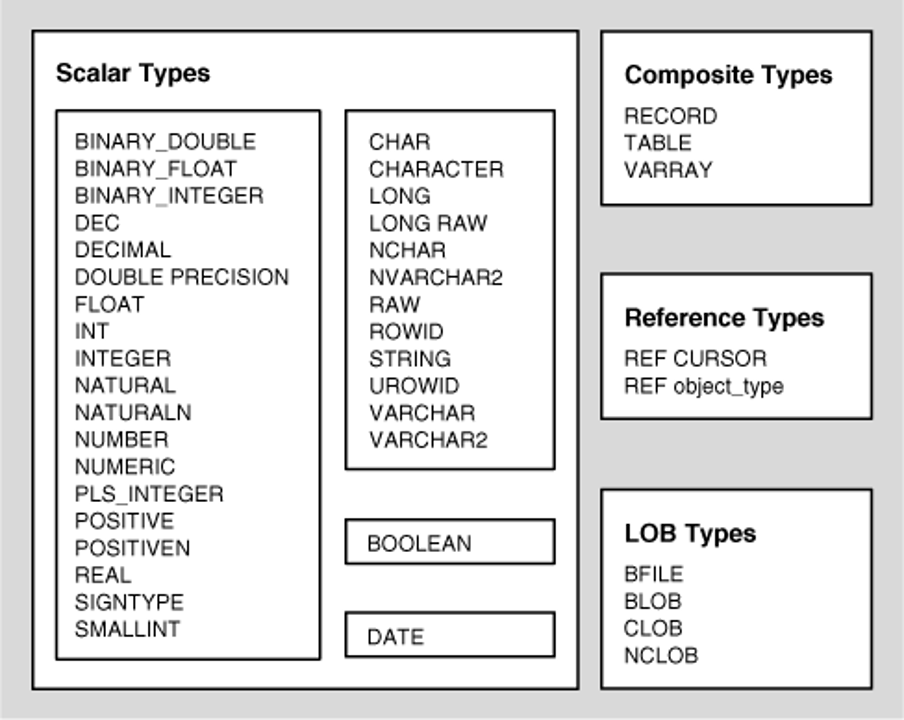
\includegraphics[width=0.60\textwidth]{../assets/img/scalar-type.png}
            \caption{Types de données scalaires}
        \end{center}
    \end{figure}
\end{frame}

\subsection{Quatre catégories}
\begin{frame}{\secname : \subsecname}
    \begin{table}[]
        \resizebox{\textwidth}{!}{%
            \begin{tabular}{|l|l|}
                \hline
                Scalaires                                                                           & \begin{tabular}[c]{@{}l@{}}Ces types sont atomiques : ce sont les types utilisés pour définir une \\ colonne d'une table\end{tabular}                                                        \\ \hline
                Composés                                                                            & Ces types comprennent plus d'un élément ou composant                                                                                                                                         \\ \hline
                Références                                                                          & Ces types permettent de définir des références vers d'autres types                                                                                                                           \\ \hline
                \begin{tabular}[c]{@{}l@{}}Grands Objets\\ (LOB = Large Binary Object)\end{tabular} & \begin{tabular}[c]{@{}l@{}}Ces types de données spécifient la localisation d'un "grand objet" \\ binaire comme une image stockée dans la base de données ou un fichier externe.\end{tabular} \\ \hline
            \end{tabular}
        }
    \end{table}
\end{frame}

\begin{frame}{\secname : \subsecname}
    \begin{enumerate}
        \item Types de données numériques
        \item Types de données "caractères"
        \item Type de données booléen
        \item Types de données \lstinline[language=plsql]!DATE!, \lstinline[language=plsql]!TIME! et \lstinline[language=plsql]!INTERVAL!
    \end{enumerate}
\end{frame}
\subsection{Types de données numériques}
\begin{frame}{\secname : \subsecname}
    \begin{itemize}
        \item \lstinline[language=plsql]!NUMBER[(P, S)]!
        \item \lstinline[language=plsql]!BINARY_INTEGER!
        \item \lstinline[language=plsql]!PLS_INTEGER!
        \item \lstinline[language=plsql]!BINARY_FLOAT! et \lstinline[language=plsql]!BINARY_DOUBLE!
    \end{itemize}

\end{frame}

\subsection{Types de données numériques NUMBER[(P, S)]}
\begin{frame}{\secname : \subsecname}
    \begin{itemize}
        \item P : nombre de chiffres significatifs
        \item S : nombre de décimales
        \item \lstinline[language=plsql]!NUMBER! possède quelques sous-types permettant une compatibilité ANSI/ISO dont, entre autres :
        \item \lstinline[language=plsql]!DEC! ou \lstinline[language=plsql]!DECIMAL! : nombre, virgule fixe, de 38 chiffres max
        \item \lstinline[language=plsql]!INTEGER!, \lstinline[language=plsql]!INT! ou \lstinline[language=plsql]!SMALLINT! : entier de 38 chiffres max
    \end{itemize}
\end{frame}
\subsection{Types de données numériques BINARY\_INTEGER}
\begin{frame}{\secname : \subsecname}
    \begin{itemize}
        \item \lstinline[language=plsql]!BINARY_INTEGER! Nombres entiers signés compris entre -2.147.483.647 et +2.147.483.647
        \item Types dérivés :
              \begin{itemize}
                  \item \lstinline[language=plsql]!NATURAL! ou \lstinline[language=plsql]!POSITIVE! : Permettent de restreindre uniquement aux valeurs non négatives (pour \lstinline[language=plsql]!NATURAL!) ou positives (pour \lstinline[language=plsql]!POSITIVE!)
                  \item \lstinline[language=plsql]!NATURALN! ou \lstinline[language=plsql]!POSITIVEN! : Idem que pour NATURAL et POSITIVE, mais n'acceptent pas la valeur nulle
                  \item \lstinline[language=plsql]!SIGNTYPE! : Retreint un entier aux valeurs -1, 0, 1
              \end{itemize}
    \end{itemize}
\end{frame}

\subsection{Types de données numériques PLS\_INTEGER}
\begin{frame}{\secname : \subsecname}
    \begin{itemize}
        \item Il est \textbf{plus performant} que \lstinline[language=plsql]!NUMBER! et \lstinline[language=plsql]!BINARY_INTEGER! qui utilisent des librairies arithmétiques
        \item Même s'il possède le même rang que \lstinline[language=plsql]!BINARY_INTEGER!, il ne se comporte pas toujours de la même manière
        \item Alors que \lstinline[language=plsql]!BINARY_INTEGER! ne génère pas une \textbf{exception} lorsqu'un dépassement de capacité intervient lors d'un calcul si le résultat est transféré dans un \lstinline[language=plsql]!NUMBER!, \lstinline[language=plsql]!PLS_INTEGER! génère bien une exception
        \item Pour des raisons de compatibilité, il est toujours possible d'utiliser \lstinline[language=plsql]!BINARY_INTEGER!, mais il est conseillé d'utiliser \lstinline[language=plsql]!PLS_INTEGER! dans les nouvelles applications

    \end{itemize}
\end{frame}

\subsection{Types de données numériques BINARY\_FLOAT}
\begin{frame}{\secname : \subsecname}
    \begin{itemize}
        \item \lstinline[language=plsql]!BINARY_FLOAT! et \lstinline[language=plsql]!BINARY_DOUBLE!
        \item Ces 2 types de données sont nouveaux depuis Oracle 10g
        \item Il s'agit de nombres floating-point de format IEEE-754 simple et double précision
        \item Ils permettent d'augmenter la performance d'applications nécessitant certains types de calculs notamment certaines applications manipulant des données scientifiques.
    \end{itemize}
\end{frame}

\subsection{Types de données numériques CHAR}
\begin{frame}{\secname : \subsecname}
    \begin{itemize}
        \item \lstinline[language=plsql]!CHAR [(maximum size [CHAR | BYTE])]!
        \item Chaînes de longueur fixe
        \item Stockage dépendant du jeu de caractères de DB
        \item Taille exprimée par défaut en bytes (maximum 32767)
    \end{itemize}
    ATTENTION : Aux jeux de caractères multi byte. On préfère \lstinline[language=plsql]!CHAR(20 CHAR)!
\end{frame}

\subsection{Types de données numériques VARCHAR2}
\begin{frame}{\secname : \subsecname}
    \begin{itemize}
        \item VARCHAR2 (maximum size [CHAR | BYTE])
        \item Chaînes de longueur variable
        \item Stockage dépendant du jeu de caractères de DB
        \item Taille exprimée par défaut en bytes (maximum 32767)
    \end{itemize}
\end{frame}

\subsection{Types de données numériques LONG}
\begin{frame}{\secname : \subsecname}
    \begin{itemize}
        \item \lstinline[language=plsql]!LONG! et \lstinline[language=plsql]!LONG RAW!
        \item Le type \lstinline[language=plsql]!LONG! est similaire à \lstinline[language=plsql]!VARCHAR2! sauf que le nombre maximum de bytes est 32760
        \item \lstinline[language=plsql]!LONG RAW! est similaire mais n'est pas interprété par le PL/SQL
        \item Les variables de type \lstinline[language=plsql]!LOB! sont destinées à remplacer les types \lstinline[language=plsql]!LONG! et \lstinline[language=plsql]!LONG RAW!
    \end{itemize}
\end{frame}

\subsection{Types de données numériques RAW}
\begin{frame}{\secname : \subsecname}
    \begin{itemize}
        \item \lstinline[language=plsql]!RAW (maximum size)!
        \item Ce type de données permet de traiter des données binaires ou des caractères en binaire.
    \end{itemize}
\end{frame}

\subsection{Types de données numériques ROWID}
\begin{frame}{\secname : \subsecname}
    \begin{itemize}
        \item \lstinline[language=plsql]!ROWID! \lstinline[language=plsql]!UROWID!
        \item De manière interne, chaque table de base de données possède une pseudo-colonne \lstinline[language=plsql]!ROWID! qui comprend une valeur binaire.  Chacune de ces valeurs (rowid) représente l'adresse de stockage de la ligne correspondante.
        \item \lstinline[language=plsql]!ROWID! permet uniquement de traiter des rowids physiques \lstinline[language=plsql]!UROWID! (rowids universels) permet de traiter les rowids physiques, logiques et "étranger", c'est-à-dire vers des tables étrangères (non Oracle).
    \end{itemize}
    \lstinputlisting[language=plsql, title=La fonction CAST permet de convertir une donnée de type rowid]{../exemples/PLSQL Chapitre 2/rowid.sql}
\end{frame}

\subsection{Types de données numériques NCHAR}
\begin{frame}{\secname : \subsecname}
    \begin{itemize}
        \item \lstinline[language=plsql]!NCHAR[(maximum size)]! et \lstinline[language=plsql]!NVARCHAR2! (maximum size)
        \item Les types de données NCHAR et NVARCHAR2 sont identiques au types CHAR et VARCHAR2 mais les données sont traitées et stockéeS au format du jeu de caractères national.
    \end{itemize}
\end{frame}

\subsection{Types de données DATE, TIME et INTERVAL}
\begin{frame}{\secname : \subsecname}
    \begin{itemize}
        \item Type \lstinline[language=plsql]!DATE!
        \item Type \lstinline[language=plsql]!TIMESTAMP [(précision)]!
        \item Type \lstinline[language=plsql]!INTERVAL  DAY [(précision)] TO SECOND [(précision)]!
        \item Type \lstinline[language=plsql]!INTERVAL  YEAR [(précision)] TO MONTH!
    \end{itemize}
\end{frame}

\section{Types de données LOBS}
\begin{frame}{\secname}
    \begin{itemize}
        \item Sont regroupés sous cette appellation tous les large objects
        \item Ils peuvent contenir des données non structurées pouvant aller jusqu'à 4 gigabytes.
        \item Nous ne les aborderons pas dans le cadre de ce cours.
    \end{itemize}
\end{frame}

\section{Structure d'un bloc}
\begin{frame}{\secname}
    \lstinputlisting[language=plsql, title=Structure d'un bloc]{../exemples/PLSQL Chapitre 2/bloc.sql}
\end{frame}

\begin{frame}{\secname}
    \begin{itemize}
        \item Une section de déclaration de variables
              \begin{itemize}
                  \item Permet de stocker des données récupérées par des instructions SQL dans les colonnes des tables.  Elles peuvent également conserver des données internes au bloc.
                        Les variables peuvent être scalaires ou composées
                        Les variables doivent être obligatoirement déclarées avant leur utilisation
              \end{itemize}
        \item Une section d'instructions
        \item Une section d'exception
    \end{itemize}
\end{frame}

\section{Déclaration de variables}
\begin{frame}{\secname}
    \lstinputlisting[language=bnf, title=Déclaration de variables]{../exemples/PLSQL Chapitre 2/bloc.bnf}
    \begin{itemize}
        \item \lstinline[language=bnf]!Nom_variable! : ce nom de variable doit être unique dans le bloc
        \item \lstinline[language=bnf]!TYPE! : le type de la variable qui peut être un type scalaire ou un type composite
        \item \lstinline[language=bnf]!CONSTANT! : La valeur de la variable est une constante qui ne sera pas modifiable dans le bloc
        \item \lstinline[language=bnf]!NOT NULL! : la variable doit obligatoirement être assignée, sinon une erreur est générée
        \item \lstinline[language=bnf]!:= VALEUR! : la variable est initialisée avec la valeur
    \end{itemize}
\end{frame}

\begin{frame}{\secname}
    \lstinputlisting[language=plsql, title=Une variable déclarée NOT NULL doit avoir une affectation d'initialisation]{../exemples/PLSQL Chapitre 2/bloc1.sql}
\end{frame}

\begin{frame}{\secname}
    \lstinputlisting[language=plsql, title=L'expression 'VCONST' ne peut pas être utilisée comme cible d'une affectation]{../exemples/PLSQL Chapitre 2/bloc2.sql}
\end{frame}

\section{Types composites ou composés}
\begin{frame}{\secname}
    \begin{itemize}
        \item Ces types de données font partie des types de données définis par le programmeur PL/SQL
        \item Parmi ces types, on retrouve également les types dérivés ou sous-types, objets de la section suivante.
    \end{itemize}
\end{frame}

\subsection{Type RECORD}
\begin{frame}{\secname : \subsecname}
    Le type de données RECORD permet de déclarer des types de variables composites.
    \begin{itemize}
        \item Un \lstinline[language=plsql]!RECORD! est l'équivalent de la définition d'un enregistrement ou d'une structure de données d'un langage de 3ème génération
        \item Il doit faire l'objet d'une déclaration d'un type de données et ensuite une variable peut être définie à l'aide de ce type
    \end{itemize}
\end{frame}

\begin{frame}{\secname : \subsecname}
    Donc, pour déclarer un RECORD, on doit passer par deux étapes distinctes :
    \begin{itemize}
        \item Déclarer un TYPE correspondant à la structure voulue
        \item Utiliser ce TYPE pour déclarer une variable
    \end{itemize}
\end{frame}

\begin{frame}{\secname : \subsecname}
    \lstinputlisting[language=plsql, title=Exemple : (cfr schéma SCOTT\, table emp)]{../exemples/PLSQL Chapitre 2/record.sql}
\end{frame}

\begin{frame}[allowframebreaks]{\secname : \subsecname}
    \lstinputlisting[language=plsql, title=Exemple : Initialisation d'un RECORD]{../exemples/PLSQL Chapitre 2/record2.sql}
\end{frame}

\subsection{Utilisation de \%TYPE}
\begin{frame}{\secname : \subsecname}
    \begin{itemize}
        \item L'attribut \lstinline[language=plsql]!\%TYPE! permet de déclarer une variable dont le type est basé sur le type d'une colonne ou d'une autre variable
        \item Les variables déclarées à l'aide de l'attribut \lstinline[language=plsql]!\%TYPE! héritent du type de données de la colonne ou de la variable référencée mais non automatiquement des contraintes (comme \lstinline[language=plsql]!NOT NULL! ou \lstinline[language=plsql]!DEFAULT!)
    \end{itemize}
\end{frame}

\begin{frame}[allowframebreaks]{\secname : \subsecname}
    \lstinputlisting[language=plsql, title=Utilisation de \%TYPE]{../exemples/PLSQL Chapitre 2/record3.sql}
\end{frame}

\begin{frame}{\secname : \subsecname}
    \lstinputlisting[language=plsql, title=ma\_variable hérite de la contrainte NOT NULL]{../exemples/PLSQL Chapitre 2/record4.sql}
\end{frame}

\begin{frame}{\secname : \subsecname}
    \lstinputlisting[language=plsql, title=ma\_variable n'hérite pas de la clause DEFAULT]{../exemples/PLSQL Chapitre 2/record5.sql}
\end{frame}

\subsection{Utilisation de \%ROWTYPE}
\begin{frame}{\secname : \subsecname}
    \lstinputlisting[language=plsql, title=Utilisation de \%ROWTYPE]{../exemples/PLSQL Chapitre 2/rowtype.sql}
    Il \textbf{n}'est \textbf{pas} nécessaire de \textbf{connaître le nom de toutes les colonnes} d'une table ni le nombre et l'ordre de ces colonnes pour effectuer une sélection.
\end{frame}

\begin{frame}{\secname : \subsecname}
    \lstinputlisting[language=plsql, title=Portée des variables]{../exemples/PLSQL Chapitre 2/rowtype2.sql}
\end{frame}

\begin{frame}{\secname : \subsecname}
    \lstinputlisting[language=plsql, title=Portée des variables : solution]{../exemples/PLSQL Chapitre 2/rowtype3.sql}
\end{frame}

\section{Conversion de types}
\subsection{Conversions explicites}
\begin{frame}{\secname : \subsecname}
    Fonction normalisée \lstinline[language=plsql]!CAST! disponible depuis Oracle 9iR2.
    \lstinputlisting[language=plsql, title=Exemple]{../exemples/PLSQL Chapitre 2/cast.sql}
\end{frame}

\subsection{Conversions implicites}
\begin{frame}[allowframebreaks]{\secname : \subsecname}
    Fonction normalisée \lstinline[language=plsql]!CAST! disponible depuis Oracle 9iR2.
    \lstinputlisting[language=plsql, title=Exemple : conversions implicites]{../exemples/PLSQL Chapitre 2/conversion-implicite.sql}
\end{frame}

\section{Types REF}
\begin{frame}{\secname}
    \begin{itemize}
        \item Les types \lstinline[language=plsql]!REF! (référence) représentent des valeurs correspondant à des pointeurs qui permettent de référencer d'autres objets du code.
        \item Certaines de ces utilisations relèvent des extensions objet-relationnelles.\footnote{Nous ne les aborderons pas.}
    \end{itemize}
\end{frame}

\section{Visibilité des variables}
\begin{frame}{\secname}
    \begin{itemize}
        \item Une variable est référencée par son nom et est visible dans le bloc PL/SQL où elle a été déclarée.
        \item Elle est visible également dans tous les blocs imbriqués dans celui où la déclaration a été faite pour autant qu'elle n'ait pas été redéfinie.
    \end{itemize}
\end{frame}
\begin{frame}{\secname}
    \lstinputlisting[language=plsql, title=Visibilité des variables]{../exemples/PLSQL Chapitre 2/visibilite.sql}
\end{frame}

\section{Opérateurs et expressions}
\begin{frame}{\secname}
    \begin{itemize}
        \item Les expressions PL/SQL sont construites en appliquant des opérateurs à des opérandes.
        \item Une opérande peut être une variable, une constante ou par exemple un littéral
        \item Les expressions sont évaluées suivant la préséance des opérateurs
    \end{itemize}
\end{frame}

\begin{frame}{\secname}
    \begin{table}[]
        \begin{tabular}{|l|l|}
            \hline
            \textbf{Opérateur}                                                                                                                                                                                & \textbf{Opération}                   \\ \hline
            **                                                                                                                                                                                                & Exponentiation                       \\ \hline
            -                                                                                                                                                                                                 & Opposé                               \\ \hline
            *, /                                                                                                                                                                                              & Multiplication, division             \\ \hline
            +, -, ||                                                                                                                                                                                          & Addition, soustraction concaténation \\ \hline
            \begin{tabular}[c]{@{}l@{}}=, \textless{}, \textgreater{}, \textless{}=, \textgreater{}=, \textless{}\textgreater{}, !=, $\sim$=, \textasciicircum{}=, \\ IS NULL, LIKE, BETWEEN, IN\end{tabular} & Comparaison                          \\ \hline
            NOT                                                                                                                                                                                               & Négation logique                     \\ \hline
            AND                                                                                                                                                                                               & Conjonction (ET Logique)             \\ \hline
            OR                                                                                                                                                                                                & OU Logique                           \\ \hline
        \end{tabular}
        \caption{Opérateurs et expressions}
    \end{table}
    \lstinline[language=plsql]!<>!, \lstinline[language=plsql]!\!=!, \lstinline[language=plsql]!\~=!, \lstinline[language=plsql]!\^=!  :  4 manière d'exprimer la différence.
\end{frame}

\begin{frame}{\secname}
    \metroset{block=fill}
    \begin{alertblock}{Important}
        PL/SQL utilise des évaluations d'expression appelées "short-circuit"
    \end{alertblock}
    Dès que le résultat de l'expression peut être déterminé, l'évaluation s'arrête
    \lstinputlisting[language=plsql, title=Ne générera pas d'erreur]{../exemples/PLSQL Chapitre 2/short-circuit.sql}
\end{frame}

\section{Logique trivalente et valeur NULL}
\begin{frame}{\secname}
    \begin{itemize}
        \item VRAI
        \item FAUX
        \item INCONNU
    \end{itemize}
\end{frame}

\begin{frame}{\secname}
    Norme SQL2 : \lstinline[language=bnf]!COALESCE (expr [, expr] ...)!
    Fonctions Oracle
    \begin{itemize}
        \item NVL
        \item NULLIF
        \item NVL2
    \end{itemize}
\end{frame}
\section{Séq. et pseudo-colonnes du PL/SQL}
\begin{frame}{\secname}
    Le PL/SQL reconnaît les pseudo-colonnes de SQL telles que \lstinline[language=plsql]!ROWID!, \lstinline[language=plsql]!CURRVAL!, \lstinline[language=plsql]!NEXTVAL!, \lstinline[language=plsql]!LEVEL! et \lstinline[language=plsql]!ROWNUM!
    \lstinputlisting[language=plsql, title=Exemple]{../exemples/PLSQL Chapitre 2/pseudo-colonne.sql}
\end{frame}

\begin{frame}[allowframebreaks]{\secname}
    \lstinputlisting[language=plsql, title=Exemple]{../exemples/PLSQL Chapitre 2/pseudo-colonne2.sql}
\end{frame}

\begin{frame}{\secname}
    \begin{itemize}
        \item \lstinline[language=plsql]!ROWNUM! permet de spécifier l'ordre dans lequel une ligne est sélectionnée dans une table.  Le premier tuple sélectionné porte le ROWNUM 1, le deuxième le
        \item \lstinline[language=plsql]!ROWNUM2! et ainsi de suite.
        \item \lstinline[language=plsql]!ROWNUM! est attribué avant l'opération de tri (\lstinline[language=plsql]!ORDER BY!)
    \end{itemize}
\end{frame}

\begin{frame}{\secname}
    \lstinputlisting[language=plsql, title=Exemple]{../exemples/PLSQL Chapitre 2/pseudo-colonne3.sql}
\end{frame}

\begin{frame}{\secname}
    \lstinputlisting[language=plsql, title=Exemple]{../exemples/PLSQL Chapitre 2/pseudo-colonne4.sql}
\end{frame}

\end{document}